% \documentclass[11pt,mathserif]{beamer}
\documentclass[11pt]{beamer}

\usepackage[english]{babel}
\usepackage{pgf}
\usepackage{amsmath,amssymb,wasysym}
\usepackage[latin1]{inputenc}
\usepackage{multirow}
\usepackage{graphicx}
\usepackage{ulem}
\usepackage{color}
\usepackage{comment}
\usepackage{hyperref}
% \usepackage{listings}
\usepackage{tabularx}

\definecolor{dred}{RGB}{200,0,0}
\definecolor{dgreen}{RGB}{0,150,0}

\mode<presentation>
{
  \useinnertheme{rectangles}
  \useoutertheme{split}
  \setbeamerfont{block title}{size={}}
  \usefonttheme{structurebold}
  \usecolortheme{Intel}
  \setbeamercovered{transparent}
}

\pgfdeclareimage[width=3.0cm]{intel-logo}{intel2}
\titlegraphic{
  \pgfuseimage{intel-logo}
}

\title[MPI+MPI]{The MPI+MPI programming model and why we need shared-memory MPI libraries}
\author[Jeff Hammond]{Jeff Hammond}
\institute[Intel Labs]{Extreme Scalability Group \& Parallel Computing Lab\\ Intel Corporation (Portland, OR)}
\date[]{26 September 2014}

\begin{document}

\frame{\titlepage}

\begin{frame}{Abstract (for posterity)}
    The MPI-3 standard provides a portable interface to interprocess 
    shared-memory through the RMA functionality. This allow applications 
    to leverage shared-memory programming within a strictly MPI paradigm, 
    which mitigates some of the challenges of MPI+X programming using 
    threads associated with shared-by-default behavior and race conditions, 
    NUMA and Amdahl's law. I will describe the MPI shared-memory capability 
    and how it might be targeted by existing multithreaded libraries.
\end{frame}

\begin{frame}{}
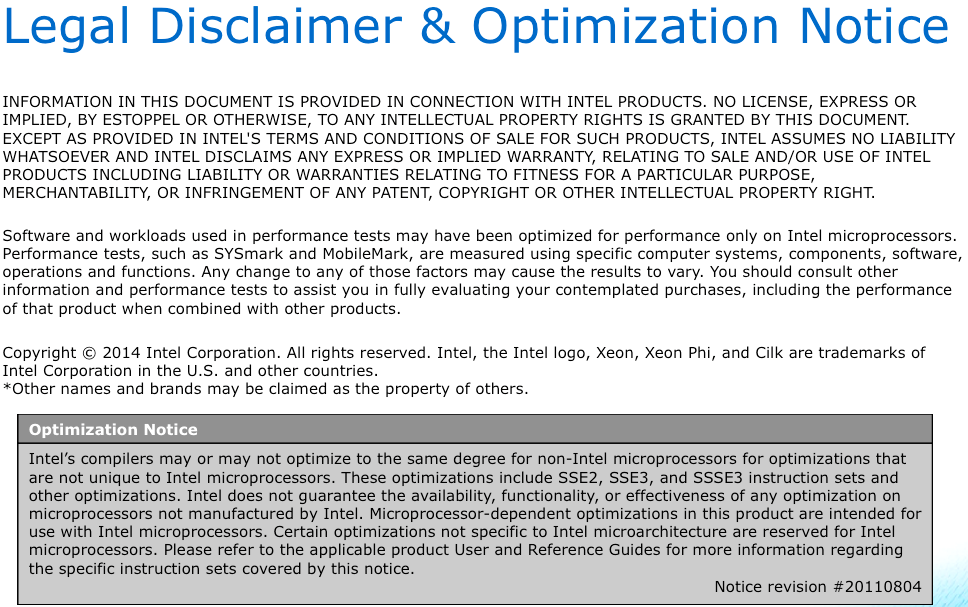
\includegraphics[scale=0.33,angle=0]{intel-legal} \
\end{frame}

\begin{frame}{Extreme Scalability Group Disclaimer}
    \begin{itemize}
        \item I work in Intel Labs and therefore don't know anything about Intel products.
        \item I work for Intel, but I am not an official spokesman for Intel.
              Hence anything I say are my words, not Intel's.
              Furthermore, I do not speak for my collaborators,
              whether they be inside or outside Intel.
        \item You may or may not be able to reproduce any performance numbers I report.
        \item Performance numbers for non-Intel platforms were obtained by non-Intel people.
        \item Hanlon's Razor.
    \end{itemize}
\end{frame}

\end{document}
